\documentclass[preprint]{JHEP3} % 10pt is ignored!

\JHEPspecialurl{http://jhep.sissa.it/JOURNAL/JHEP3.tar.gz}
\usepackage{graphicx}
\usepackage{amsmath,amssymb}
\usepackage{cite}
\usepackage{multirow}

%\newcommand{\DF1A}{\Delta F_{1,A}}
%\newcommand{\DF1V}{\Delta F_{1,V}}
%\newcommand{\Dphill}{\Delta \phi_{ll}}
\newcommand{\be}{\begin{eqnarray}}
\newcommand{\ee}{\end{eqnarray}}
\newcommand{\ttb}{t \bar{t}}

\title{Constraining top-Z coupling through $t\bar{t}Z$ production at the LHC}

\author{Raoul R\"ontsch \\ Fermilab, Batavia, IL 60510, USA \\
  Email: \email{rontsch@fnal.gov} }
\author{Markus Schulze}


\received{\today} 		%%
%\revised{}
\accepted{\today}		%% These are for published papers.


\preprint{}

\abstract{We constrain top-Z coupling through ttbZ at LHC.}

\begin{document}
%\maketitle
\section{Introduction}
 Pheno motivation: LHC a top factory, new top measurements; possibility of measuring top couplings; ttbZ $\to \nu \nu$ as background to MET searches for stops. \\
 Previous NLO calc (w/o top or Z decay): LMMP, KTP \\
 Prev. analysis of top-Z couplings: Baur et al, Berger et al \\
 Comparison with indirect constraints on top-Z coupl \\
 Single top+Z \\

\section{Outline of calculation}
\subsection{NLO calculations}
OPP, C-S dipoles, top decay at NLO, NWA for tops and Z + Refs \\
Leptonic, inclusive variables so no need for parton showering \\
Checks: poles, factorization, alpha-param \\
Comparison with KTP, LMMP - cross-secs, distr \\

\subsection{Top-Z coupling}
Definition of top-Z couplings - vector, axial-vector, left and right handed \\
Focus of D=4 operators -- D=6 for later (unclear how to implement unitarity for such operators) \\
Definition of DF1V and DF1A

\section{Results}
\subsection{NLO Results}
Four distr incl scale bounds (incl at least one of a decay product) at LO, NLO\\
Comparison with NLO + LO decay \\
Comparison with 0+1 jet from MadGraph using CKKW merging \\
Acceptance function = $\sigma_{\mathrm{incl}} / \sigma_{\mathrm{cuts}}$ at LO, NLO\\
Point out large k-factor with cuts than with fully inclusive \\

LO and NLO cross sections for acceptance cuts given in eq.~\ref{}
\be
  \sigma_{\ttb Z}^\mathrm{LO} &= 3.80^{+1.31}_{-0.94}~\mathrm{fb},
  \quad\quad\quad
  \sigma_{\ttb Z}^\mathrm{NLO} &= 5.32^{+0.78}_{-0.74}~\mathrm{fb}
\\
% 
  \sigma_{\ttb Z}^\mathrm{LO} &= 3.80^{+34\%}_{-25\%}~\mathrm{fb},
  \quad\quad\quad
  \sigma_{\ttb Z}^\mathrm{NLO} &= 5.32^{+15\%}_{-14\%}~\mathrm{fb}
\\
% 
  \sigma_{\ttb Z}^\mathrm{LO} &= 3.98 \pm 28\% ~\mathrm{fb},
  \quad\quad\quad
  \sigma_{\ttb Z}^\mathrm{NLO} &= 5.34 \pm 14 \%~\mathrm{fb}
\ee
Results are represented in three ways (need to pick one).
We also calculate the cross section without acceptance cuts and find
\be
  A^\mathrm{LO} = \frac{\sigma_{\mathrm{cuts}}^\mathrm{LO}}{\sigma_{\mathrm{total}}^\mathrm{LO}} = 27.2 \% ,
  \quad\quad\quad
  A^\mathrm{NLO} = \frac{\sigma_{\mathrm{cuts}}^\mathrm{NLO}}{\sigma_{\mathrm{total}}^\mathrm{NLO}} = 30.5 \%.
\ee

\subsection{Top-Z coupling results}
Constraints from $t\bar{t}Z$ cross-section from CMS \\
Dphill distr with LO and NLO scale bands, and two(three?) non-SM coupl\\
$\sigma_{NP|} / \sigma_{SM}$ a la Berger, 0907.2191 \\
Description of analysis Binned log likelihood, how we handle scale uncertainty (cf. Lykken et al) \\
alpha plots - LO, NLO, rescaled (k-factor and reduced scale uncertainty) LO at 30, 300, 3000 fb-1\\
Dphill distr normalized to $t\bar{t}$ cross-section  - 1 uncertainty from k-factors at 30, 300, 3000\\

\section{Conclusion}
Future work: extension to dim 6 operators, incl single top + Z results, more advanced analysis techniques (e.g. MEM), e+e- collider.
%


\acknowledgments
We acknowledge conversations with A.~Gritsan.



\appendix
\section{plots}
Temporariy repository for plots.


\begin{figure}[h]
\centering % \begin{center}/\end{center} takes some additional vertical space
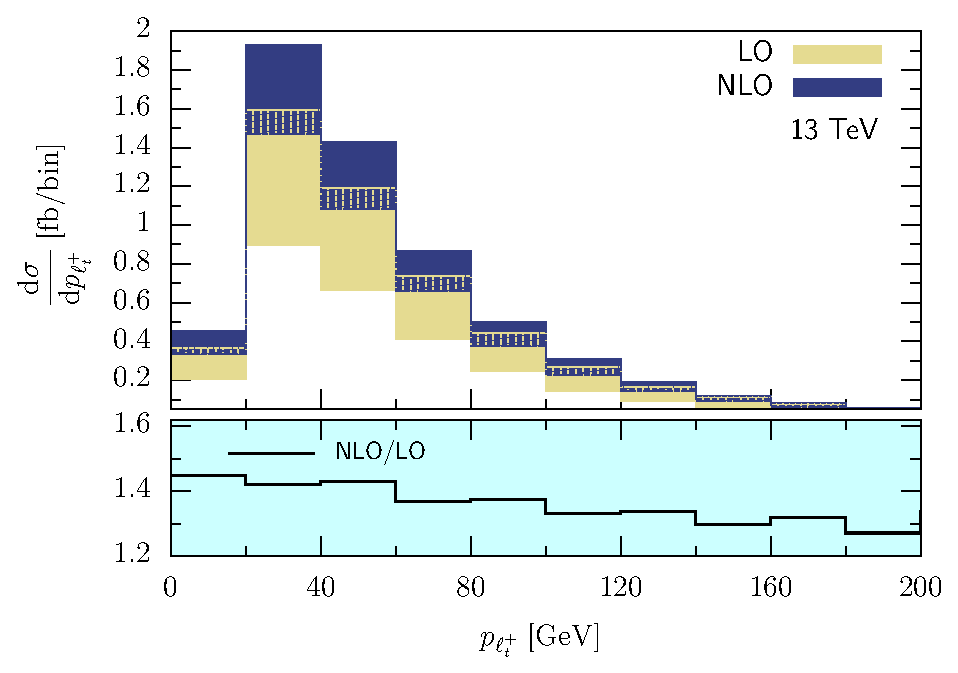
\includegraphics[width=0.45\textwidth]{./LHC_53_Fig01.eps}
\hfill
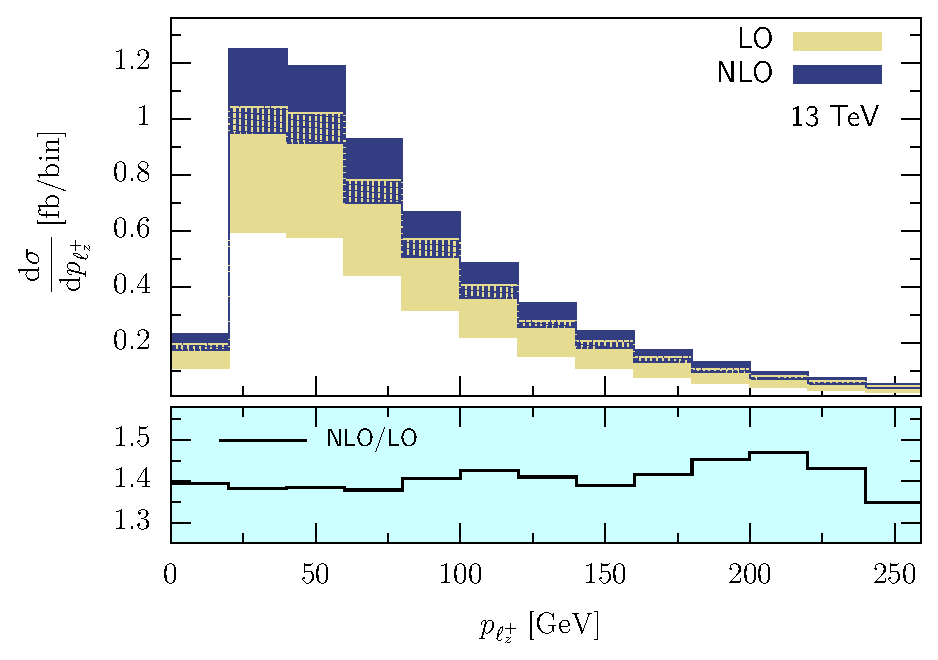
\includegraphics[width=0.45\textwidth]{./LHC_53_Fig03.eps}
\caption{\label{fig:i} Caption here.}
\end{figure}


\begin{figure}[h]
\centering % \begin{center}/\end{center} takes some additional vertical space
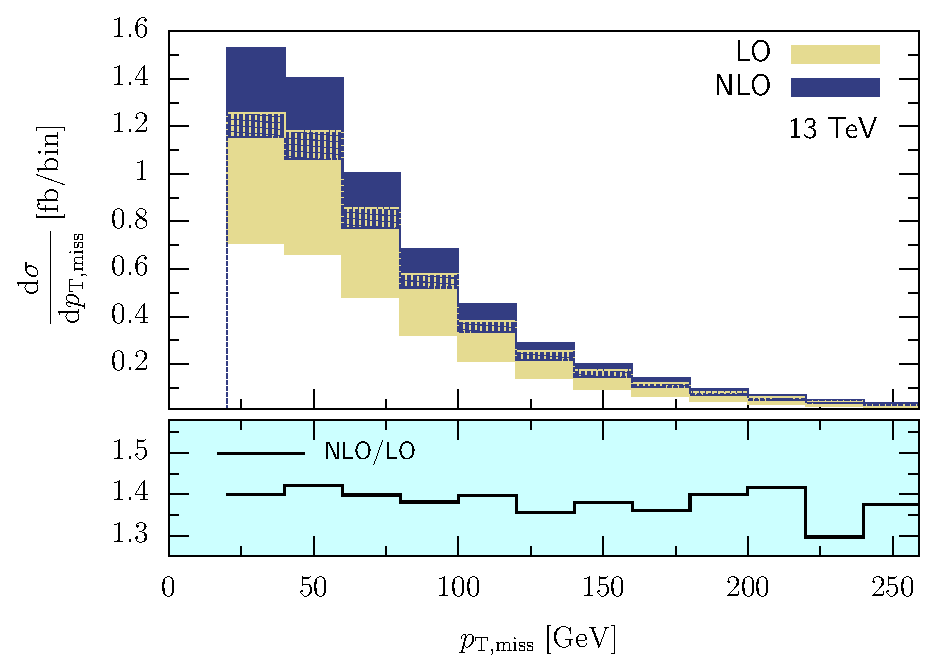
\includegraphics[width=0.45\textwidth]{./LHC_53_Fig08.eps}
\hfill
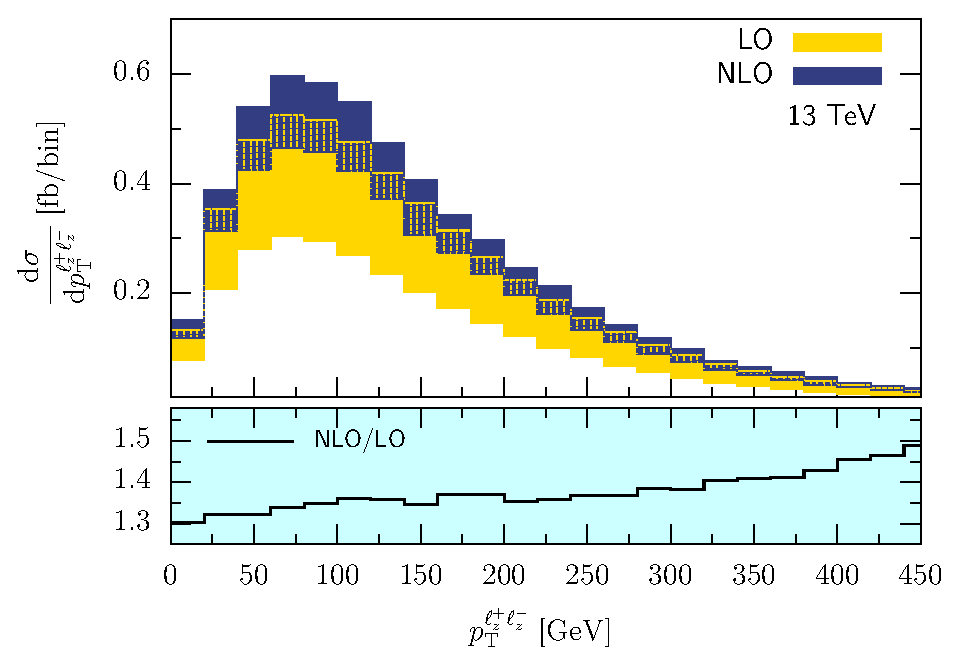
\includegraphics[width=0.45\textwidth]{./LHC_53_Fig12.eps}
\caption{\label{fig:i} Caption here.}
\end{figure}



\begin{figure}[h]
\centering % \begin{center}/\end{center} takes some additional vertical space
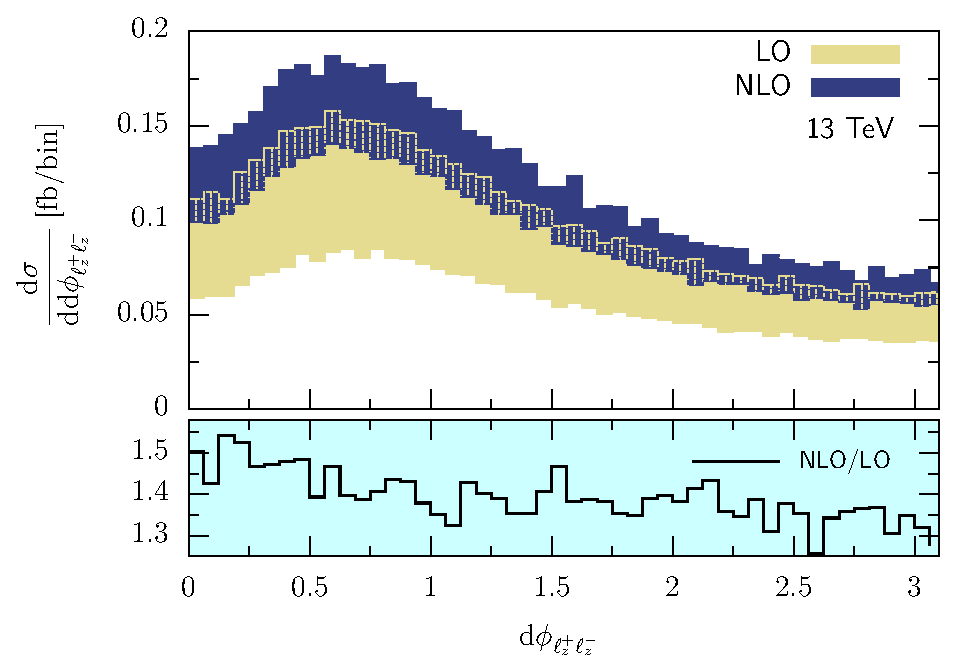
\includegraphics[width=0.45\textwidth]{./LHC_53_Fig17.eps}
\hfill
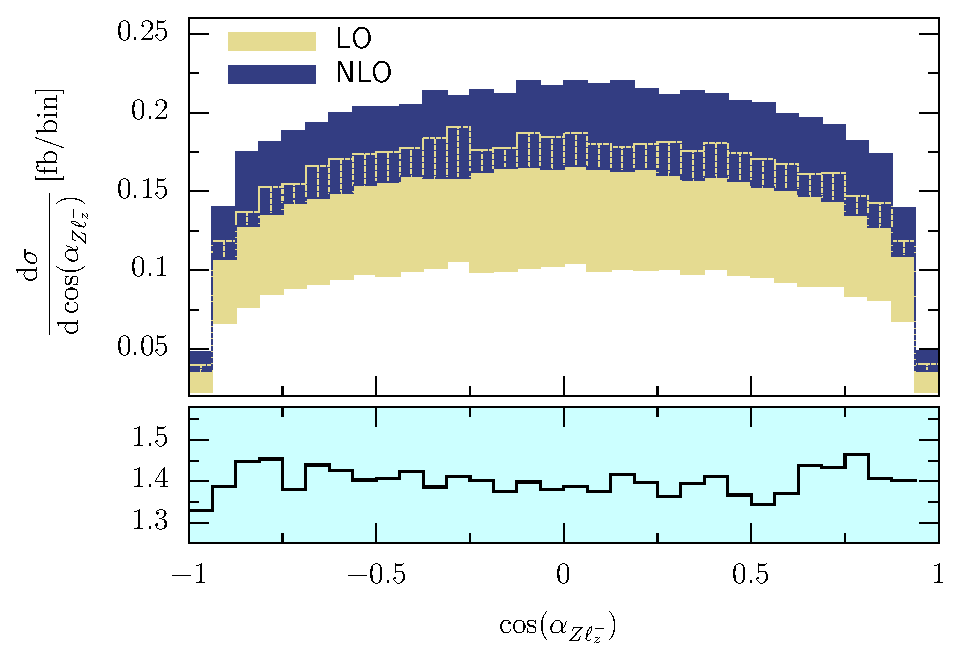
\includegraphics[width=0.45\textwidth]{./LHC_53_Fig18.eps}
\caption{\label{fig:i} Caption here.}
\end{figure}




\begin{figure}[h]
\centering % \begin{center}/\end{center} takes some additional vertical space
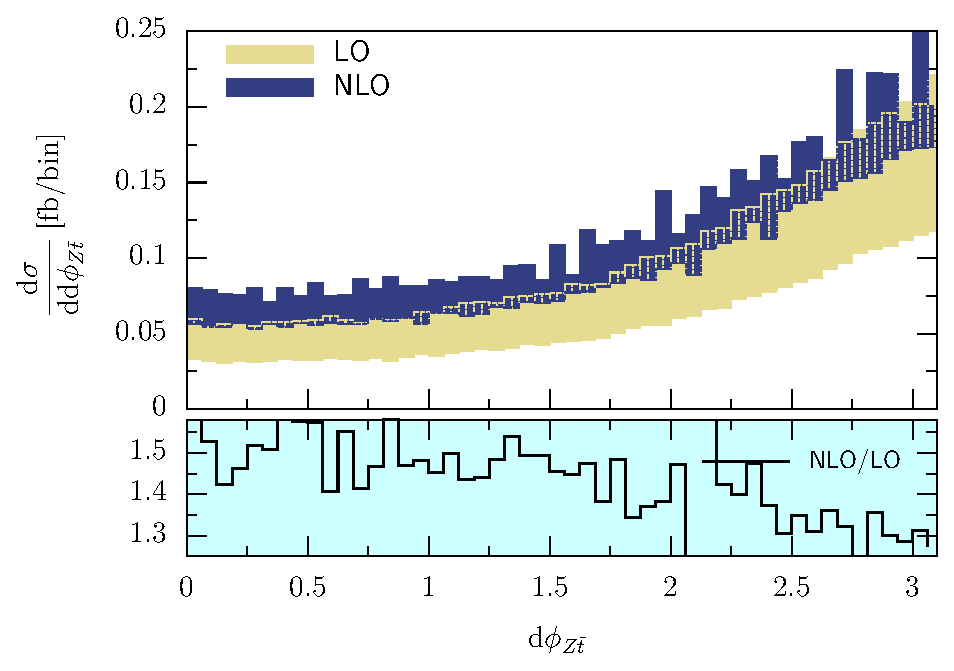
\includegraphics[width=0.45\textwidth]{./LHC_53_Fig19.eps}
\caption{\label{fig:i} Caption here.}
\end{figure}




\begin{thebibliography}{99}

%\cite{Campbell:2013yla}
\bibitem{Campbell:2013yla} 
  J.~Campbell, R.~K.~Ellis and R.~Rontsch,
  %``Single top production in association with a Z boson at the LHC,''
  Phys.\ Rev.\ D {\bf 87}, 114006 (2013)
  [arXiv:1302.3856 [hep-ph]].
  %%CITATION = ARXIV:1302.3856;%%


\end{thebibliography}

\end{document}








